%!TEX root = thesis.tex
\chapter{Probabilistic Timing Attack against to Snoopy Cache Coherency}
In this chapter of the thesis, we proposed a probabilistic attack to increase evasion probability of malware against to snoopy cache coherence protocol on tightly coupled systems with write back cache policy. We briefly explained the issue we can encounter during implementation of the cache oriented obfuscation method with the snoopy coherent systems. The snoopy cache coherency protocol's internals have already been mentioned in background studies chapter; however, we assumed through whole section that all coherence operations are atomic, and contention between processes are not subject. Yet, They are not close to be atomic; and moreover, the latency is sometimes enough long to process and to complete whole gadget or whole malware. In order to exploit this contention, we methodized a probabilistic race condition attack. 

As a brief and in other words, instead of giving an absolute obfuscation, we proposed a method which probably obfuscates malware, and this probability depends on the systems design and gadgets' processing overhead. On the other hand, this value gives us a quantitative rate, but if our concern is signature based detection methods, signatures' value can be measured with qualitative approaches rather than quantitative ones, e.g. some signature like port number or IP address are treasury.  Yet, the quantity of signature is certainly another value to measure efficiency, especially when we relate binary codes and signature detection.
\todo[inline]{Add more details about how lazy they are}

\section{The Issue}
Cache coherency is a term and discipline arisen from the incoherent states of caches due to parallel computing. It does not need multi processor environment. For incidence, sometimes, DMA devices can be enough to emerge it. In tightly coupled systems, because of the usage of caches to increase performance, it is highly possible to falling into an incoherency state. We also mentioned much more details in background studies chapter. in this chapter, the term of "stale data" is used to describe globally\footnote{In local frame, it concerns the relationship between the CPU and cache values rather than between caches. } the data which is not reflected for most current or synchronized value in the system(included with other caches and memories). In order to synchronize stale data and provide coherency between caches, cache coherency protocols and policies are used between caches. As we mentioned, most of  protocols and policies need networks between each other and logical operator per cache controller. There are many methods to provide coherency between caches and one of the most known and capable one is snoop mechanism. 

Snoopy cache coherency mechanisms provide synchronization with a bus watch mechanism in the system bus. These mechanisms imply that cache must first request the data from any other caches, before it request from the memory. The implementation of the snoop mechanism is vice versa, but works as well, as same.Cache generally watches the bus and record activities, arise exception in case of coherency problem(when it is likely to fall incoherent states).\cite{Jim2007} There is generally an interconnector to organize snoopy cache protocols, and filter useless communication. 

Moreover, the nature of the cache organization which we use commonly is lazy. The mean of lazy is they do not update the modified block and values until they evict and replace it with other cache block. The reason why they are lazy is obvious, the efficiency optimisations. If they write every modification directly memory as well as cache\footnote{It is salso  mentioned in background studies as write through policy}, it will consume most of the available bandwidth. The main essence how we keep our data in a cache as like as private memory is arisen from this laziness, because we anticipate and controls the cache line evictions and replacements. However, we cannot simply say write-through caches are perfectly coherent because of the reasons explained in Chapter 3. For example, $CacheA$ read address $x$, and then, $CacheB$ read address $x$. If $CacheA$ write address $x$ with Write-Thought policy, the value in $CacheB$ is still stale.

With perfect coherent caches, we can not exploit private caches to use as private memory (see also. NUMA); hence, we can't evade anything from one CPU to another as we did in the previous chapter. Namely, there is no difference between disk to memory and disk to cache obfuscation. Even though the highest workspace which you deobfuscate your code is cache, cache are synchronizing each other. This coherence gives ability to anti-malware scanning other caches and detecting signature.
\section{Solution}
	Let's assume we have a tightly coupled multi processor test bed system, and it has one CPU reserved to scan memory for malware detection, and another CPU is occupied by malware itself. Their caches are snoopy coherent with an interconnection network.  They could use any of protocols which we mentioned in background studies e.g. MOESI, MESI, MSI. Let's also assume that the malware which present in the second CPU's cache is designed as we defined in previous chapter. It has prewarmed cache as we described and started to deobfuscate and run the code. The presumption is the $CACHE 2$`s cache blocks is accessible by $CPU1$ as well as any other CPUs. However, the access and synchronization of any stale data is not that simple. It is presumed as atomic, but it is not, and worst of all, tightly coupled systems are heterogeneous with cache coherency, because the distance to memories are not equal and systems are not homogeneous. This heterogeneousness comes with different access times to the memories. Especially MOESI protocol is much more heterogeneous because it works as semi-NUMA(Non uniform Memory Architecture) type cache i.e. a modified cache block can be moved around various caches without updating main memory. Secondly, cache controllers rule are not really elastic. When an address is touched by a CPU, it fetches whole block in order to exploit spacial locality and increase performance\footnote{Sometimes they wait for feeding CPU until fetch it all, sometimes feed CPU as soon as possible depending on algorithm.}. We actually exploited throughout whole chapter two weaknesses which are horizontal directional cache fetching attribute and synchronization latency and heterogeneous access time of snoopy caches.
\subsection{Horizontal Directional Cache Fetching}
In computer architecture conventions, we arrange instructions into memory space, incrementally, and then, we can prefetch them before they run. Also, we are tent to use the space around we recently accessed. It is called spacial locality and we mentioned about it more deeply in background studies. For this reason, we cache mechanisms works horizontally. It fetches a particular size of memory in the same time, and put it a cache block. Besides, cache blocks are the smallest addressable memory spaces; therefore, it makes caches more simpler, faster\footnote{After an amount of memory, it could decrease performance.\cite{ComputerArchCoursera} }and cheaper. Accordingly, Fetching and eviction operations are handled as line-based namely horizontally. 
	\begin{figure}[h!]
	    \centering
	    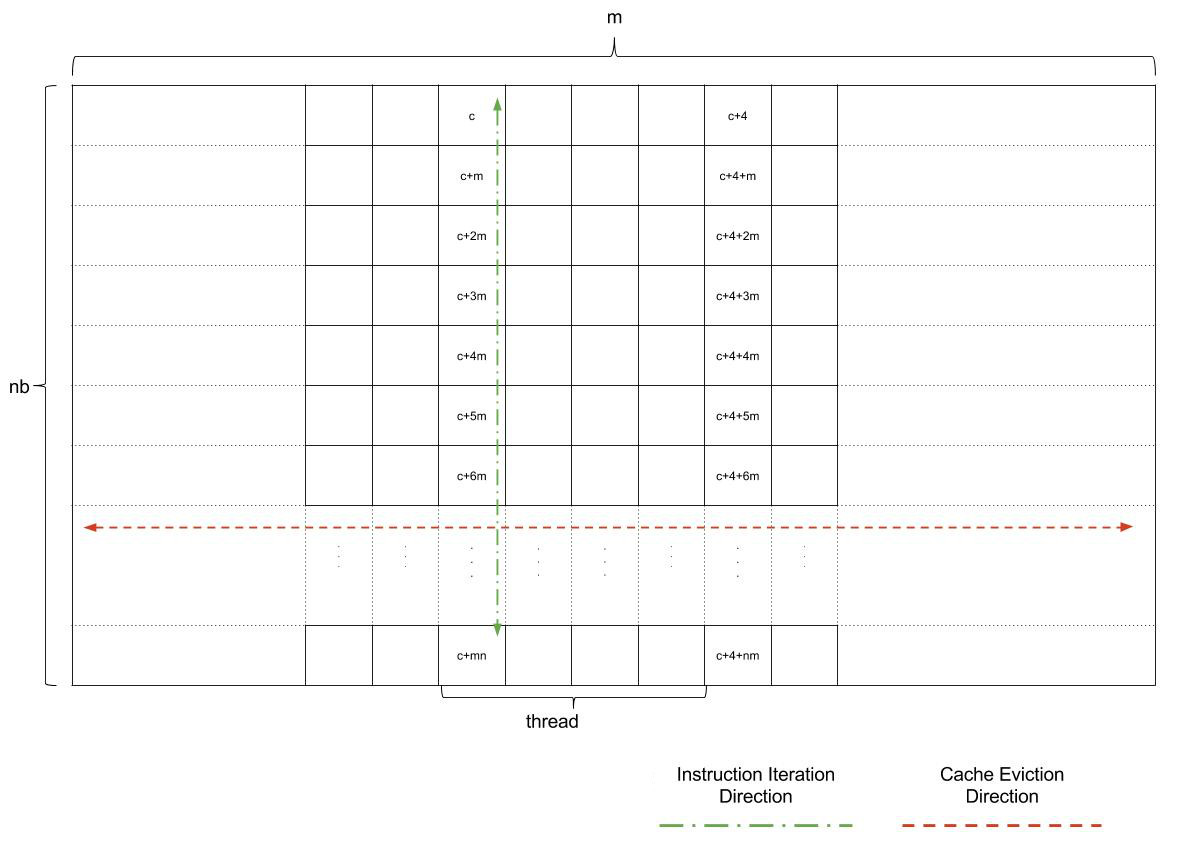
\includegraphics[width=1\textwidth]{img/vertical_instruction_iteration.jpg}
	    \caption{Directional Exploitation}
	    \label{fig:veriticaldirection}
	\end{figure}
In figure \ref{fig:veriticaldirection}, we showed data fetching direction and its contrast with our instruction iteration direction approach. As we mentioned many times, but in order to emphases it one more time, instruction sequence normally increments one by one. Yet, in our approach it iterate as in equation 5.1. $m$ is the cache block size, and $n$ is the number of cache block line in the whole cache. $nb$ is number of line which is allocated to body of our gadget as mentioned in previous chapter, so this figure is a frame of cache in which obfuscated part of our malware allocated. Let's say $c$ is the initialization point of our malware. When $i$ is the number of instruction on the queue, $I(i)$ gives us the location of instruction in the memory; thereby, in the cache. 
\begin{equation}
	I(i)=m*(i\bmod{(nb)})+((\left \lfloor i/nb \right \rfloor*thread)+c)\bmod{m}\\ 
\end{equation}
$thread$ value in the cache is step number between the vertical blocks. In order to generate a function which onto(bijective) the cache frame, equation 5.2 must be provided, because after it overflow mod function, it will uses just the one next block which previously used and go on until end. It is obvious that $tread$ should be smaller than $m$, yet it is already in mod and $i$ must be smaller than total size. 
\begin{equation}
	\forall\: m\bmod thread = 1\ :\  I()\ is\ bijective\ function
\end{equation}
Yet, Why do we iterate institution sequence  vertically? Indeed, we assumed that anti-malware scans horizontally from $CPU1$ above, because it is faster. For example, our code starts from $c$ and our second instruction in $c+m$, with purpose of scanning from $CPU1$ in this order, it should  fetch first the line of $c$ into $Cache2$, and then, it should fetches the line of $c+m$, and so forth. In the perfect world, with atomic instruction to fetches whole cache line and without latency, it could be race condition free approach, but in real systems, it is not. We will combine this attack with latency problem in the next sections.
\subsection{Synchronization Latency of Snoopy Caches}
One of the famous myth on the computer science and design is that tightly coupled parallel architectures are mostly considered as symmetric systems, but if we look more closer, the caches usage and moreover cache usage with coherency protocols and network makes them quite asymmetric and preforce them to be heterogeneous. Processors could have same properties and be arranged in symmetrical, but if they can't give same throughput in an time interval, we can't call them homogeneous\footnote{In order to prevent this, there are systems which avoid to use caches, when they are sharing data. Because of the symmetry of cache processor relationship, they keeps their symmetric design themselves.}. 


\subsubsection{Latency Calculation}
	\begin{figure}[h!]
	    \centering
	    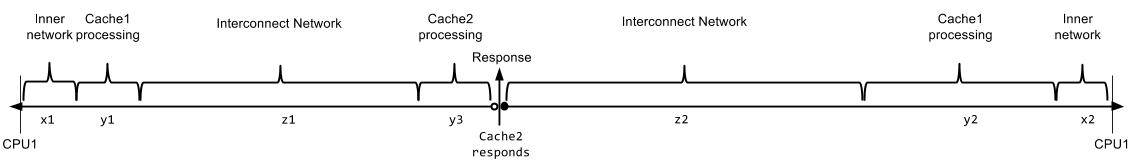
\includegraphics[width=1.1\textwidth]{img/timing_diagram.jpg}
	    \caption{The Time Line of the Fetching Cache Line which is Used by Another Cache}
	    \label{fig:timeline}
	\end{figure}
In figure \ref{fig:timeline}, we showed a representational illustration of cache line requesting process which is used in another cache, and labelled latency types with $x$ for inner network latency, $y$ for cache processing latency, $z$ for overall interconnection latency. As seen in figure \ref{fig:timeline}, the throughout latency for synchronization process with another cache is showed in equation 5.3. However, the latency of direct reaching to the cache is showed in equation 5.4 which is obviously shorter\footnote{This formulas are valid for the simple systems showed in figure \ref{fig:tightlycoupled}}. 
\begin{equation}
L_{s}=x_{1} + y_{1} + z_{1} + y_{3} + z_{2} + y_{2} + x_{2}
\end{equation}

\begin{equation}
L_{d}=x_{1} + y_{d} + x_{2}
\end{equation}
All this latency variables is depending on many different factors which we can calculate them in theory, but which is difficult to estimate in practice. $x$ variables are the latencies between CPU and cache. It is tent to be really short, because $L1$ cache and CPU should be designed so close. Mostly $x_{1} = x_{2}$, yet it is not certain. The reason is write buffer and pipelined CPU makes it case depended. Generally, most of the latency comes from the queue of cache which also related to writers block and pipelined architecture as we mentioned in background studies. $y$ variables are cache's logical response latencies. As we mentioned, It depends on cache size, associativity, line size and logical operations complexity. In this example, we have one layer cache, but most systems use multi layer caches. For each layer, it adds more overhead. In brief, caches are as fast as how simple they are.\footnote{Their design affect performance a lot, but they are mostly SDRAM instead of DRAM or switch based registers} However, there is no doubt that most important and game changer latency is $z$ namely, interconnection network latency. 
	\begin{figure}[h!]
	    \centering
	    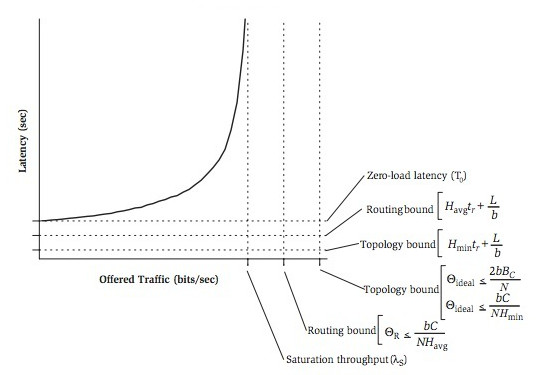
\includegraphics[width=1.1\textwidth]{img/latency_graph.jpg}
	    \caption{Interconnector Latency Versus Offered Traffic \cite{0122007514}}
	    \label{fig:latencyvsofferedtraffic}
	\end{figure}
 Mostly, lack of bandwidth is considered as the only reason of network latency, whereas there are many other factor and problems. Nevertheless, it is one of the most important source of latency. Bandwidth is the rate of the data can transmitted from point $a$ to point $b$ in a given time, but originally, it was the number of wire in width of buses. This definition ignores the clock speed contrast with current definition because the speed of wire is related with speed of light and resistance of the wire, but instead, the things which limit it is the performance of source and receiver. The bandwidth could be formulated as $ b = n * f$ where n is width of the channel and f is clock speed. Surprisingly, if our message is smaller than channel width, bandwidth can not effect latency because if we have 100 bit bandwidth, then it carries 20 and 100 bit in the same time. Notable the interconnection networks' costs are routing, serialization/deserialization, link traversal latencies\cite{0122007514}. We already have mentioned about their details; still, it is good to shortly recall that serialization and deserialization are processes to converting messages to given channel bandwidth and could be shown as $ sd = L / b $ where $L$ is length of message and $b$ is bandwidth. Therefore, overall latency can be measured with formula 5.5.
\begin{equation}
T_{0}=\sum_{k=1}^{minr}tr_{k}+\sum_{k}^{minc}D_{k}/v_{k}+L/b
\end{equation}
In this equation, $minr$ and $minc$ denote the minimum number of router and channel between point $a$ and $b$. $tr$ denotes time consumed during routing process, while $D/v$ denotes distance divided by velocity. The easy way to calculate $T_{0}$ for each flit is $T_{0} = T_{head} + L/b$ because $\sum_{k=1}^{minr}tr_{k}+\sum_{k}^{minc}D_{k}/v_{k}$ is calculated one and only one time in pipelined networks as have been mentioned. If it is not pipelined, the latency could be measured by formula 5.6 or if it was store and forward flow control instead of cut-through as shown in equation 5.5, the latency could be measured by formula 5.6 (see more details \cite{0122007514}). 
\begin{equation}
T_{0}=(\sum_{k=1}^{minr}tr_{k}+\sum_{k}^{minc}D_{k}/v_{k})*L/b
\end{equation}
\begin{equation}
T_{0}=(\sum_{k=1}^{minr}tr_{k}+\sum_{k}^{minc}D_{k}/v_{k})+(\sum_{k=1}^{minr}*L/b)
\end{equation}
However, $T_{0}$ is not a general latency function, and it is very special status of networks which is also called zero-load latency.  Zero-load latency is the lowest bound of the latency where there is no contention between packets. In figure \ref{fig:latencyvsofferedtraffic}, a generic latency vs offered traffic curve is showed. Although they are the most accurate way to measure and determine ultimate performance, and we are using discrete event simulation to draw them. Theoretic latency bounds, which are topological and routing, and their corresponding throughputs are showed in figure. In formula 5.4, 5.5 and 5.6, zero latency values are all shown with minimum routing hops which means topology bounded zero latency, but actual zero-load latency, $T_{0}$ in figure, incorporates the constraints of topology along with actual performance, routing, flow control and line traversal latency\cite{0122007514}. As have seen obviously, if you increase the contention between packets through increasing offered traffic, the latency grows about exponentially. It is one of the most important factor support our proposes and encourage us to implement because of the fact that roughly loading memory and storing back to the hard disk\footnote{It is basically dumping memory} produce remarkable traffic which can lead considerable latency.

\subsubsection*{Simulation Result}
	\begin{figure}[h!]
	    \centering
	    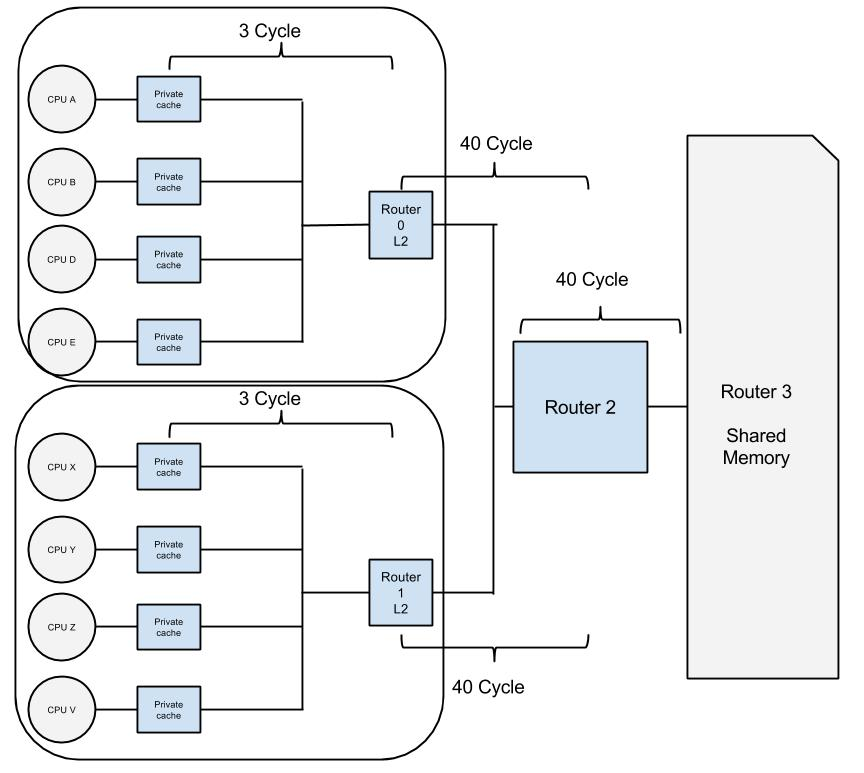
\includegraphics[width=0.8\textwidth]{img/simulation.jpg}
	    \caption{Our Simulation Topology\cite{0122007514}}
	    \label{fig:simulation}
	\end{figure}
An accurate simulation is definitely one of the most important tools for analyzing interconnection networks and exploring design tradeoffs. The reason why we are using simulations instead of real systems is a bit similar with theoretic physic. There are many noises on information we gathered from real systems and they are extremely expensive and difficult to implement. Even one of the most acknowledged books about interconnection network, which is called "Principles and Practices of Interconnection Networks" repeatedly emphasizes that designer's intuition is the most important factor to design better performance on interconnection networks\cite{0122007514}. This book has a simulation tool freely available at http://cva.standford.edu/\cite{jiang2013detailed}. Even though, every processor company invests their years and efforts to design better simulator, this tool is quite simple and totally free licensed. However, it is not designed for coherency purpose, so its model designed in flit level and includes many topologies and routing algorithms. Indeed, it can give us some important cues and ideas. 

We designed it with an example topology which we use in multiprocessing systems. It is the inheritor topology of Fat tree. In figure \ref{fig:simulation}, the topology is shown which has two processors, 3 routers\footnote{Though we said 3 routers, we used in figure and topology design file 4 router. That is due to lack of simulation tools. We tried to give a latency between router 3 and shared memory} and shared memory. This designed is influenced by one of the most known ARM chips Samsung EXYNOS 5420. This latency values are rounded numbers, but they are close values which we obtained the concerned chip\footnote{we used CPU-Z program to measure cache latencies.}. One way channel length is about 3 cycles from L1 cache controller to L2 cache controller, 40 cycles from L2 cache controller to L4 cache controller. This contrast could be because of the difference between in-chip out-chip communication and also the complexity of caches internal operation. We assumed the routing delay is about 2 cycles, even though it could be a bit more. We used 1 cycle credit delay for flow control.

The injection rate of simulation is the number of packets which it injects every cycle time. The book claims average rate is 0.15, but we consider that it is enormously high for our experiment. As we have said, injection rates could be really high during memory dumping; however, it could be decreased, if scanner avoids bad programming practice and exploit cache performance feature, it could be around one store and one load operation request  for each cache block from upper layer cache. If we take this into consideration, we assumed the injection rate 2 and 4 for each 100 cycles. It is also good to assume it lower for any cases. 

One of the other important value about our experiment is the character of our generated traffic. We used a uniform traffic generator which means every nodes talk with each other. However, it is not actually appropriate for our attack. In our example, scanner $CPUA$ talks a lot, and other CPUs talks nominal, but $CPUX$ attacker CPU does not load or store, after it initializes. We can implement our own traffic generator for this simulator in the future. This simulator is also highly adaptive and extensible with plugins.

In implementation of our topology, we decided to design two different modes to emphasize contention over network, which are small topology and crowed topology. In the small topology experiment, we assumed there are just two active nodes, three active routers and one shared memory in the network and they are the ones which connected to $CPUA$ and $CPUX$. In this example, latency is mostly based on distance and pure logical complexity, rather than contention of routing or bandwidth. In the second experiment, we designed the crowded topology which has four nodes connected to $router0$ four nodes connected to $router1$, and they are all connected to $router2$, and also we presumed there are two "slave nodes" which might be DMA devices and one GPU connected to $router2$.

\begin{table}[h]
\begin{tabular}{|l|c|c|c|c|}
	\hline
                  & \begin{tabular}[c]{@{}c@{}}Packet latency\\ Min/Avg/Max\end{tabular} & \begin{tabular}[c]{@{}c@{}}Network latency\\ Min/Avg/Max\end{tabular} & \begin{tabular}[c]{@{}c@{}}Flit latency\\ Min/Avg/Max\end{tabular} & Hops Avarage \\ \hline
Crowded 2\%            & 164/68045/171627                                                     & 13/417/1487                                                           & 13/353/1487                                                        & 2.04442      \\ \hline
Small 2\%            & 8/72/216                                                             & 8/72/216                                                              & 8/72/216                                                           & 2.30611      \\ \hline
Crowded 4\%            & 15698/178598/458108                                                  & 13/410/1736                                                           & 13/353/1736                                                        & 2.04591      \\ \hline
Small 4\%            & 8/322/1273                                                           & 8/129/376                                                             & 8/129/376                                                          & 2.33081    \\ \hline
\end{tabular}
\caption{Simulation Results Comparison}
\label{table:simulation}
\end{table}

The result of the simulation is added in appendix B, and briefly showed in table \ref{table:simulation}. We made four experiment with two different topology and two different injection rate as have been mentioned. For more details, you can check appendix B. We present in this table three different kind of latencies. Flit latency is a simple latency time required from the beginning of flit till end. Latency of a packet is measured from the time its head flit is generated by the source to the time its tail flit is consumed by the destination. Obviously, flit latency is the delay time for transferring a flit from one node to next node which routers applied as node in this case. The contrast with network latency and flit latency is tricky. Network latency is flit latency plus extra serialization and routing costs. Hops average is the average number of hops every flits traversed (except source hop) during experiment. It could give an idea about distribution of message. As you can see, the average hop number is lower on crowed topology because nodes under the same router can talk with each other i.e. $CPUA$ can send a message to $CPUB$ as well as $CPUX$ does $CPUY$. The value which we concern is packet latency, because packets are smallest meaningful communication object. To provide coherency, cache controllers communicate with packets between each other. 

As you can see, on an typical crowded network, average latency varies around $68000$ cycle to $178000$ cycles. If we assume clock cycle is around $1 GHZ$, $100000$ cycle is about 0.1 second absolute time. On the other hand, it is around 72 to 322 on small sized topology. However, if we concern the communication between $CPUA$ and $CPUX$ it is at least $40$ cycles + $40$ cycles + (3 * routing costs) + $3$ cycles + $3$ cycles = $92 cycles$ because of the distance. It means that the latencies we need to concern is above average and close to upper bound because $CPUA$ and $CPUX$ is one of the farthest couple.

It is hard to point an exact average latency value for any system, even if we are exactly sure about target system. The contention is the most important factor for latency. In order to increase the chance of our attack we could use noise production methods from other nodes, but because of its character and highly detectability, it is not recommended, still the scanning and storing processes produces enough latency due to high dependency of memory load store operation. 

\subsection{Overall Explanation of the Timing Attack}
\begin{figure}[h!]
    \centering
    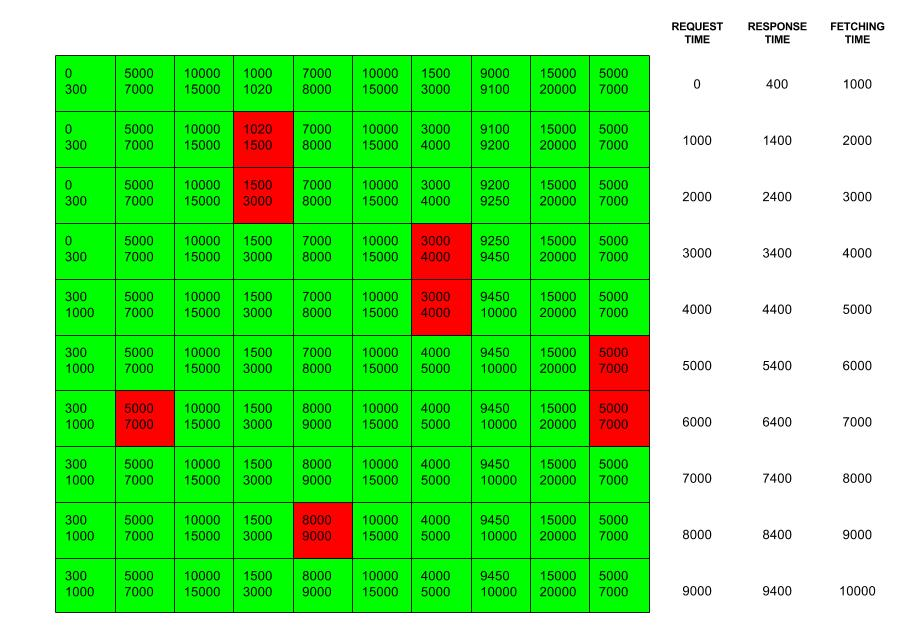
\includegraphics[width=1\textwidth]{img/overall_timing_attack.jpg}
    \caption{The illustration of cache and time Interaction is showed with leaked portion of obfuscated data}
    \label{fig:overall}
	\end{figure}
	Let's presume again we have a malware which is designed as we have proposed in chapter 4 and we have the same system which we have designed in figure \ref{fig:simulation}. Then, the malicious malware is loaded from non-volatile memory e.g. hard-disk to memory obfuscated and it loaded to the cache which belongs $CPUX$. It arranged the structure of cache as have been mentioned in previous proposal. It have been designed as same as it was so far. The point in this situation is we have a memory scanner and dumper application which works in another cache (in this example it is the cache belongs $CPUA$.), and we assume $CPUA$ has coherent cache with $cache x$. This coherency can be provided with snoopy cache coherency through one of the protocols of MEOSI, MESI, MSI. After malware loads the obfuscated code from the memory to the cache, it is allocated as shared state in MSI or exclusive state in MOESI and MESI. It is good to know that it is not going to transmit to modified or owned state until it deobfuscate it. The things which we don't want to share is plain data, and lets call this action as leakage. When we de obfuscate the code, its block in the cache transmits to modified state. Then, if an scanner cpu, $CPUA$, request the block line which we deobfuscate, the long adventure of synchronization starts.

	Our stepped control flow approach has already be proposed as a solution for coherency because instead of whole cache block line leakage, it will lose one step during even theoretical atomic snapshot, and strongly probably it is not going to be meaningful to be signature; however, this stepped approach is not completely good because of its complexity and the effect of that complexity over stub which increase the chance of detectability. The attack we have proposed in this chapter is starting with arranging the steps(more flexible steps, more likely to be smaller gadgets) to the cache vertically as shown in figure \ref{fig:veriticaldirection}, with given formulas 5.3, 5.4. 

	The example which we illustrated is shown in figure \ref{fig:overall}. The time zero on this example is representing the time of the first moment which actually scanner reach the memory location of malware, while the malware's process is flowing. We have another latency assumption here the latency of $x1+y1+z1+y3$ in figure \ref{fig:timeline} is equal to 400 cycle time and $z2+zy2+x3$ is equals to 600 cycle time. The second one is longer because first one which request the cache line is a packet with a header flit, and tail flit. On the other hand response packet comes with whole cache line\footnote{the experiments we made with Booksim 2.0 showed this values as nominal network latency for the topology we designed}. The response time, which we showed in figure \ref{fig:overall} and mentioned in figure \ref{fig:timeline}, is the moment, after it received load request from $CPUA$ and responded it with the cache line. In this moment, cache line is not in modified state, since it is transmitted to the owned or shared state. The interesting point is here that if $CPUX$ manages to write back obfuscated value in place of plain value, then the cache controller of can synchronize this value before scanner detect or store it\footnote{this synchronization could be quite fast with MOESI protocol because $cacheX$ probably allocated it with owned state}. 

	If you look at figure \ref{fig:overall} again, the time intervals which they are deobfuscated and plain showed in the boxes. These intervals are the vulnerable moments for leakage. However, they are ordered vertically, so they can not be fetched in the some time from another cache. The leaked boxes are showed also in the figure. They are the cache block whose line is synchronized, when they are deobfuscated. For example; the first red block on the second line is sent to $cacheA$ at 1400 cycle time, and it was using from 1020 till 1500 cycle time. Therefore it is leaked. However, there are just 8 boxes over 100 boxes overall.

\subsubsection{Overall Obfuscation Rate Calculation}
In order to calculate overall obfuscation rate, we can use formula below. 

\begin{equation}
	\frac{totalblock-leakedblock}{totalblock}
\end{equation}

However, it gives you an quantitative rate which does not represent whether it is evasion or not. Evasion is more depended on qualitative approaches rather than the percent age of obfuscated block because the signature which we uses for detection is generally some strings such as IP addresses or domain names. Of course, the instruction structure is important especially with control flow graph detection, still majority is string searching. The leakage from these strings could be fatal for evasion, even though their size are relatively smaller. Nevertheless, it can imply a general perception about how successful obfuscation we have. It is not going to be same for even particular system and latency, but the mean of many attempts is reliable. So lets formulate it for better accuracy like below:
\begin{equation}
	\frac{\sum_{1}^{n}\frac{totalblock-leaked}{totalblock}}{n}
\end{equation}

In order to increase obfuscation complexity, the exotic kind of settlement structure can be proposed as vertical settlement have been proposed e.g. crosswise, curved so forth. Complexity is not good security practice, but can be useful and necessary for obfuscation. This attack, which we proposed  throughout chapter, will absolutely work with some degree of evasion, but the thing which determines its success is latency of interconnetion network and so, their designs and their logical complexity.

\section{Pitfalls, Limitations and Fallacies}
Even though our methods are novel and theoretically possible, we skip many details in this chapter. For example, the deadlock and live locks in interconnection networks are one of the most common problems. In order to break coherency, they could be useful to exploit, however, it is another attack and vast area. However, it is theoretical likely to appear, if there are to node which share same resource in the same time. 

We also did not mention so much about coherency protocols in this chapter, but they could be useful or problematic depending on case. For example, while you are running around malware cache, if there is another CPU who try to scan you cache, it cat not simply modify cache. Instead, it will demand right of modify for cache line, then other cache controller invalidate the line and then respond to the cache which want to write. It require a lot of time\footnote{As we mentioned in background studies chapter it is a lot more flexible}, and it is the thing can be resulted with deadlock. In addition, this latency could be useful to detect a process of detection. Namely, if there is a difference between write latency, it could be signature of coherence request, but it can't be useful for prevention against scanning.

In the example we showed in figure \ref{fig:overall}, the malware's processing flow spread around the whole cache equivalently, but the most of common processing flow of regular malware are normally comprised with long period of time delay algorithms or watch dog instructions. In these cases, the only thing scanner can obtain is useless instruction which can not be useful to identify malware.

We did not try to calculate process overhead in this chapter, but it is all about contention and race between latency and process overhead. The reason why we did not is that In modern computer architecture, it is quite difficult to calculate it because of the pipelined and out-of-ordered processors. They can process many instruction in the same time concurrently and simultaneously. We should be aware of this, when we design malware. Arranging different kind of instructions sequentially makes it more faster and concurrent, even if we have one core. You can see more details of this architecture in figure \ref{fig:blockdiagram}\footnote{Computer architecture: The quantitative approach book is the one of the best resource about them\cite{ComputerArchCoursera}}.

Memory management and protection units are also the subjects which we never mention in this chapter, yet they are making this attack a bit more possible because they produce extra traffic and extra logical complexity and worst of all, they increase traffic exponentially, however, today, there are interconnector chips for multi processing system which handle memory management itself i.e. Arm CCI 400, 500.